% Options for packages loaded elsewhere
\PassOptionsToPackage{unicode}{hyperref}
\PassOptionsToPackage{hyphens}{url}
%
\documentclass[
  12pt,
  a4paper,
]{article}
\usepackage{amsmath,amssymb}
\usepackage[]{mathptmx}
\usepackage{setspace}
\usepackage{iftex}
\ifPDFTeX
  \usepackage[T1]{fontenc}
  \usepackage[utf8]{inputenc}
  \usepackage{textcomp} % provide euro and other symbols
\else % if luatex or xetex
  \usepackage{unicode-math}
  \defaultfontfeatures{Scale=MatchLowercase}
  \defaultfontfeatures[\rmfamily]{Ligatures=TeX,Scale=1}
\fi
% Use upquote if available, for straight quotes in verbatim environments
\IfFileExists{upquote.sty}{\usepackage{upquote}}{}
\IfFileExists{microtype.sty}{% use microtype if available
  \usepackage[]{microtype}
  \UseMicrotypeSet[protrusion]{basicmath} % disable protrusion for tt fonts
}{}
\usepackage{xcolor}
\usepackage[top = 25mm,bottom = 25mm,left = 25mm,right = 25mm]{geometry}
\usepackage{graphicx}
\makeatletter
\def\maxwidth{\ifdim\Gin@nat@width>\linewidth\linewidth\else\Gin@nat@width\fi}
\def\maxheight{\ifdim\Gin@nat@height>\textheight\textheight\else\Gin@nat@height\fi}
\makeatother
% Scale images if necessary, so that they will not overflow the page
% margins by default, and it is still possible to overwrite the defaults
% using explicit options in \includegraphics[width, height, ...]{}
\setkeys{Gin}{width=\maxwidth,height=\maxheight,keepaspectratio}
% Set default figure placement to htbp
\makeatletter
\def\fps@figure{htbp}
\makeatother
\setlength{\emergencystretch}{3em} % prevent overfull lines
\providecommand{\tightlist}{%
  \setlength{\itemsep}{0pt}\setlength{\parskip}{0pt}}
\setcounter{secnumdepth}{-\maxdimen} % remove section numbering
\pagestyle{headings}
\newlength{\cslhangindent}
\setlength{\cslhangindent}{1.5em}
\newlength{\csllabelwidth}
\setlength{\csllabelwidth}{3em}
\newlength{\cslentryspacingunit} % times entry-spacing
\setlength{\cslentryspacingunit}{\parskip}
\newenvironment{CSLReferences}[2] % #1 hanging-ident, #2 entry spacing
 {% don't indent paragraphs
  \setlength{\parindent}{0pt}
  % turn on hanging indent if param 1 is 1
  \ifodd #1
  \let\oldpar\par
  \def\par{\hangindent=\cslhangindent\oldpar}
  \fi
  % set entry spacing
  \setlength{\parskip}{#2\cslentryspacingunit}
 }%
 {}
\usepackage{calc}
\newcommand{\CSLBlock}[1]{#1\hfill\break}
\newcommand{\CSLLeftMargin}[1]{\parbox[t]{\csllabelwidth}{#1}}
\newcommand{\CSLRightInline}[1]{\parbox[t]{\linewidth - \csllabelwidth}{#1}\break}
\newcommand{\CSLIndent}[1]{\hspace{\cslhangindent}#1}
\ifLuaTeX
\usepackage[bidi=basic]{babel}
\else
\usepackage[bidi=default]{babel}
\fi
\babelprovide[main,import]{brazilian}
% get rid of language-specific shorthands (see #6817):
\let\LanguageShortHands\languageshorthands
\def\languageshorthands#1{}
\ifLuaTeX
  \usepackage{selnolig}  % disable illegal ligatures
\fi
\IfFileExists{bookmark.sty}{\usepackage{bookmark}}{\usepackage{hyperref}}
\IfFileExists{xurl.sty}{\usepackage{xurl}}{} % add URL line breaks if available
\urlstyle{same} % disable monospaced font for URLs
\hypersetup{
  pdftitle={Equilíbrio da estrutura intraurbana},
  pdfauthor={Arthur Bazolli Alvarenga e Prof.ª Rosa Lívia Montenegro},
  pdflang={pt-BR},
  hidelinks,
  pdfcreator={LaTeX via pandoc}}

\title{Equilíbrio da estrutura intraurbana}
\usepackage{etoolbox}
\makeatletter
\providecommand{\subtitle}[1]{% add subtitle to \maketitle
  \apptocmd{\@title}{\par {\large #1 \par}}{}{}
}
\makeatother
\subtitle{Aula 10 (semana 12) - ECO075}
\author{Arthur Bazolli Alvarenga e Prof.ª Rosa Lívia Montenegro}
\date{Janeiro de 2023}

\begin{document}
\maketitle

\setstretch{1}
\hypertarget{introduuxe7uxe3o}{%
\section{Introdução}\label{introduuxe7uxe3o}}

Esta nota de aula é baseada principalmente no capítulo 7 de O'Sullivan
(2012), no capítulo 2 de Brueckner (2011) e nos capítulos 2 a 4 de
Bertaud (2018).

Agora que já estudamos os modelos canônicos da economia urbana, podemos
compreender melhor como as forças econômicas atuam dentro das cidades. O
propósito desta aula é mostrar \textbf{como a estrutura dos centros
urbanos evoluiu ao longo do tempo}, frente às mudanças observadas nas
tecnologias de transporte, de construção e de informação e nas
preferências dos agentes econômicos. Mas, antes, vamos recapitular as
premissas básicas dos modelos que desenvolvemos e os fatos estilizados
da economia urbana.

\hypertarget{premissas-buxe1sicas}{%
\subsection{Premissas básicas}\label{premissas-buxe1sicas}}

Os modelos urbanos são construídos em cima do arcabouço da
microeconômico, separando os agentes econômicos entre indivíduos (ou
famílias)\footnote{no inglês, usa-se o termo \emph{households},
  comumente traduzido como famílias} e firmas.

O \textbf{dilema dos indivíduos} é entre consumir o \textbf{máximo de
espaço} residencial possível e ter o \textbf{menor custo de transporte}
possível. No geral, o custo de transporte é modelado como função linear
da distância ao trabalho, mas pode ser entendido como um \textbf{custo
de oportunidade} do tempo e dinheiro perdidos no deslocamento
casa-trabalho.

Já as firmas desejam maximizar o lucro gastando o mínimo possível com
seus fatores, como salários, \textbf{custos de transporte} e terra. Um
detalhe fundamental é que as \textbf{economias de aglomeração}, quando
presentes, podem aumentar os lucros da empresa. Assim, se uma
localização promove essas economias, a empresa pode preferir arcar com
custos maiores de aluguel para aproveitá-las.

Economias de aglomeração ocorrem quando a concentração de agentes
econômicos próximos aumenta o retorno econômico. Um exemplo é quando
indústrias de um mesmo setor se instalam em uma mesma cidade e, tendo
fornecedores similares, viabilizam a instalação de uma cadeia de
suprimentos na vizinhança que reduz os custos de aquisição dos insumos.
São os \textbf{arranjos produtivos locais} (APLs), como o da mineração
no quadrilátero ferrífero de Minas Gerais ou o polo automobilístico do
ABC Paulista.

Se enxergarmos as cidades como mercados de trabalho, fica fácil
identificar outras duas fontes de economias de aglomeração. Um deles
está relacionado à \textbf{inovação}: a alta concentração de pessoas em
uma região tende a aumentar as interações e a criar uma rede de troca de
informações que impulsiona novas ideias. Por exemplo, ex-funcionários de
uma empresa estabelecida podem transferir o conhecimento adquirido para
uma nova empresa, como ocorreu e ainda ocorre no Vale do Silício.

\begin{quote}
\emph{``Por exemplo, os primeiros usuários de planilhas eletrônicas em
microcomputadores (no início dos anos 1980) eram principalmente
contadores e analistas financeiros. O uso de planilhas logo ficou comum
em todos os setores da economia, mas o} spillover \emph{aconteceu
primeiro em grandes cidades, partindo do MIT em Cambridge,
Massachusetts, onde foi originalmente inventado. Spillovers de
conhecimento são responsáveis por economias de aglomeração (ou seja,
economias que aumentam a produtividade devido à rápida disseminação de
novas ideias porque um grande número de trabalhadores está em contato
próximo)``}. Bertaud (2018, 21, tradução nossa)
\end{quote}

Por fim, o terceiro fator diz respeito à especialização: a oferta de
trabalho das grandes cidades permite obter maiores graus de
especialização, pois é nelas que a mão de obra especializada encontra
demanda por esse tipo de trabalho. É uma situação do tipo ``ovo ou a
galinha'' (ou \emph{endógena}, como dizemos na economia): empresas
atraem trabalhadores capacitados para a cidade, mas cidades com
trabalhadores especializados também atraem empresas que demandam
trabalhos sofisticados. Isso dá origem a um ciclo
\textbf{retroalimentador} que gera altos níveis de especialização da mão
de obra e, assim, a economia local pode atingir níveis maiores de
produção.

\hypertarget{fatos-estilizados}{%
\subsection{Fatos estilizados}\label{fatos-estilizados}}

De acordo com o dicionário \emph{online} Oxford Reference, fatos
estilizados são ``observações empíricas usadas como ponto inicial para a
construção de teorias econômicas. Um fato estilizado deve ser verdadeiro
no geral, mas não necessariamente em todos os casos''. Em outras
palavras, fazemos generalizações a partir da realidade para construir as
teorias econômicas, mas devemos lembrar que elas são uma percepção geral
e não uma verdade absoluta ou imutável. Como veremos a seguir, as
dinâmicas urbanas mudam ao longo do tempo, mas alguns princípios válidos
parecem se sustentar ao teste do tempo.\footnote{Fonte:
  \url{https://www.oxfordreference.com/display/10.1093/oi/authority.20110810105949304;jsessionid=1E3AE33B3DE49AAD939B92F3FB7F5AE8}}

\hypertarget{comportamento-das-firmas}{%
\subsubsection{Comportamento das
firmas}\label{comportamento-das-firmas}}

No setor terciário, quando o contato físico é essencial ---como o
comércio, profissionais da saúde, advogados--- as firmas tendem a se
concentrar no CBD da cidade. Já se o contato não faz tanta diferença,
como em \emph{call centers} e outras atividades operacionais, a empresa
otimizadora tende a procurar locais mais baratos, como outros subcentros
ou mesmo em outros países. Algumas atividades dão origem a subcentros
especializados fora do CBD: exemplos em Juiz de Fora são a Av.
Deusdedith Salgado (concessionárias) e a Rua Henrique Vaz (ferro velho e
peças automotivas).

Já para as indústrias, as economias de aglomeração também são
importantes, mas a tendência não é se concentrar no CBD. Em vez disso, a
tendência é uma concentração nos principais \textbf{nós de transporte},
já que os produtos são distribuídos para diversos locais, dando origem a
outros subcentros.

\begin{quote}
\textbf{\emph{Os subcentros matam o centro?}} Não. Eles são
complementares, e atraem diferentes atividades econômicas de acordo com
a localização otimizadora para cada uma.
\end{quote}

\hypertarget{comportamento-dos-indivuxedduos}{%
\subsubsection{Comportamento dos
indivíduos}\label{comportamento-dos-indivuxedduos}}

Ao contrário das firmas, os indivíduos estão mais dispersos. No entanto,
observamos que muitas famílias preferem trocar espaço e tranquilidade
pela comodidade de morar perto do centro. Se observarmos os dados de
densidade populacional e de preços dos imóveis em várias cidades do
mundo, verificamos um \textbf{gradiente} de preços e de
\textbf{densidade} populacional ao redor dos CBDs, mesmo que a tendência
nos últimos 40 ou 50 anos tenha sido de espraiamento.

Bertaud e Malpezzi (2003) analisaram o perfil da área construída de
cerca de 50 cidades e identificaram o decaimento exponencial de
densidade a partir do centro proposto pela teoria. Para as 12 cidades
exemplificadas abaixo, o grau de ajuste (\(R^2\)) de uma função do tipo
\(densidade = e^{\beta dist\_cbd}\) ficou acima de 0,80 para todas as
cidades, com exceção do Rio de Janeiro. De fato, como notam os autores,
a topografia do Rio ---morros, florestas, baía de Guanabara--- é uma das
razões por trás do desvio ao fato estilizado.

\begin{figure}

{\centering 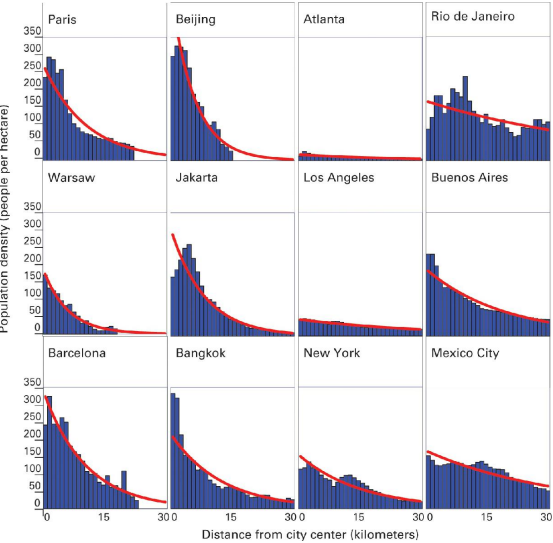
\includegraphics[width=7.68in]{src/images/bertaud_density} 

}

\caption{\label{fig:density} densidade ao redor do mundo. Fonte: Bertaud (2018)}\label{fig:density}
\end{figure}

\hypertarget{padruxf5es-de-deslocamento}{%
\subsubsection{Padrões de
deslocamento}\label{padruxf5es-de-deslocamento}}

O terceiro fato estilizado diz respeito à locomoção de pessoas nas
cidades. Os principais deslocamentos são do tipo casa-trabalho (ou
comutação, do inglês \emph{commuting}), ainda que não sejam os únicos.
Em cidades \textbf{monocêntricas}, os deslocamentos tendem a ser
\textbf{radiais} e fortemente \textbf{pendulares}, ou seja:
concentram-se na direção bairro-centro no pico da manhã e na direção
oposta no pico da tarde. Por outro lado, cidades mais
\textbf{policêntricas} têm padrões mais \textbf{diversos}. As cidades
americanas, por exemplo, são bastante espraiadas e, na média, 44\% dos
deslocamentos se dão entre os subúrbios e não em direção ao CBD
(O'Sullivan 2012). A imagem abaixo ilustra os padrões de deslocamento
para diferentes tipologias de estrutura urbana:

\begin{figure}

{\centering 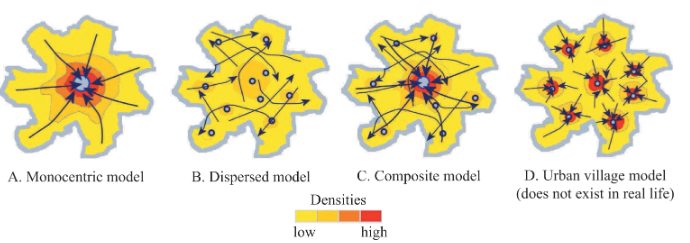
\includegraphics[width=0.8\linewidth]{src/images/bertaud_commuting} 

}

\caption{\label{fig:commuting} Padrões de deslocamento. Fonte: Bertaud (2018)}\label{fig:commuting}
\end{figure}

Entender os padrões de deslocamento é importante não só para planejar a
rede de transportes da cidade, como também para investigar o
\textbf{acesso a oportunidades}; ou seja, o grau de facilidade (ou
dificuldade) que os cidadãos encontram para encontrarem trabalho e
chegar a escolas, hospitais e demais equipamentos.

\hypertarget{a-ascensuxe3o-da-cidade-monocuxeantrica}{%
\section{A ascensão da cidade
monocêntrica}\label{a-ascensuxe3o-da-cidade-monocuxeantrica}}

Nos \textbf{primórdios}, as cidades já seguiam um padrão monocêntrico,
geralmente ao redor de construções religiosas, governamentais ou
militares. Na Europa medieval, era comum que a urbe fosse limitada por
muros, para protegê-la de invasões, e a vida fora dos muros se
restringia a pequenas vilas e atividade agrícola.

Os modos de transporte se restringiam às \textbf{embarcações} ---para
exportar mercadoria e enviar ao interior por rios---, e à \textbf{tração
animal}, para deslocamento dentro da cidade, transbordo ao porto e
atingir o interior onde não era possível por via fluvial (mais lento e
custoso). Com isso, mesmo dentro da cidade, o \textbf{custo de
transportar} mercadoria era uma barreira muito grande que regia a
decisão locacional das firmas. Isso também se aplicava aos
\textbf{indivíduos}, restritos sobretudo ao deslocamento \textbf{a pé
e}, quando muito, força animal.

Assim, a atividade \textbf{manufatureira} era restrita ao
\textbf{centro} das cidades e zonas portuárias, enquanto os
trabalhadores deveriam morar perto (para padrões atuais) de seus
trabalhos.

A partir da Revolução Industrial, surgiram tecnologias que permitiram às
cidades crescer tanto para os lados quanto para cima. Uma das principais
foi a \textbf{locomotiva a vapor}: o desenvolvimento das ferrovias
permitiu que as indústrias alcançassem mais mercados, mas também,
permitiu o surgimento de um novo \textbf{padrão espacial}:
\emph{clusters} industriais perto das estações. A localização no centro
continuava atrativa para as indústrias, mas não era indispensável como
antes dos trens.

\hypertarget{inovauxe7uxf5es-no-transporte-urbano}{%
\subsection{Inovações no transporte
urbano}\label{inovauxe7uxf5es-no-transporte-urbano}}

Para entender a importância dos meios de transporte no equilíbrio
espacial urbano, é importante ter em mente que o \textbf{tamanho} de uma
cidade costuma ser limitado pela distância que é possível percorrer em
uma hora a partir do CBD. É claro que há pessoas que gastam mais de uma
hora para chegar ao trabalho, mas a maior parte da mancha urbana se
concentra dentro desse limite. Assim, quando as únicas possibilidades
disponíveis eram andar a pé ou por tração animal, a \textbf{área viável}
de uma cidade era bem menor do que hoje, quando temos diversos meios de
transporte disponíveis.

Uma dessas inovações foi o \textbf{bonde} elétrico (e seu antecessor, o
ômnibus, puxado por cavalos). Ao aumentar a acessibilidade de locais
mais afastados ao centro, o bonde reforçou o padrão monocêntrico: como
as linhas levavam a periferia às zonas centrais, o comércio e a
indústria se desenvolveram ao longo desses corredores. Ainda no século
XIX, surgiu o trem metropolitano (\textbf{metrô}): criado em Londres
como uma extensão subterrânea para a rede ferroviária atingir o centro
da cidade, o modelo foi replicado ao redor do mundo e é, sem dúvidas, um
importante promotor de acessibilidade.

A imagem abaixo mostra a rede de bondes de Belo Horizonte, por volta dos
anos 1950: é possível notar um padrão, irradiando a partir da Praça 7, o
CBD da cidade.

\begin{figure}

{\centering 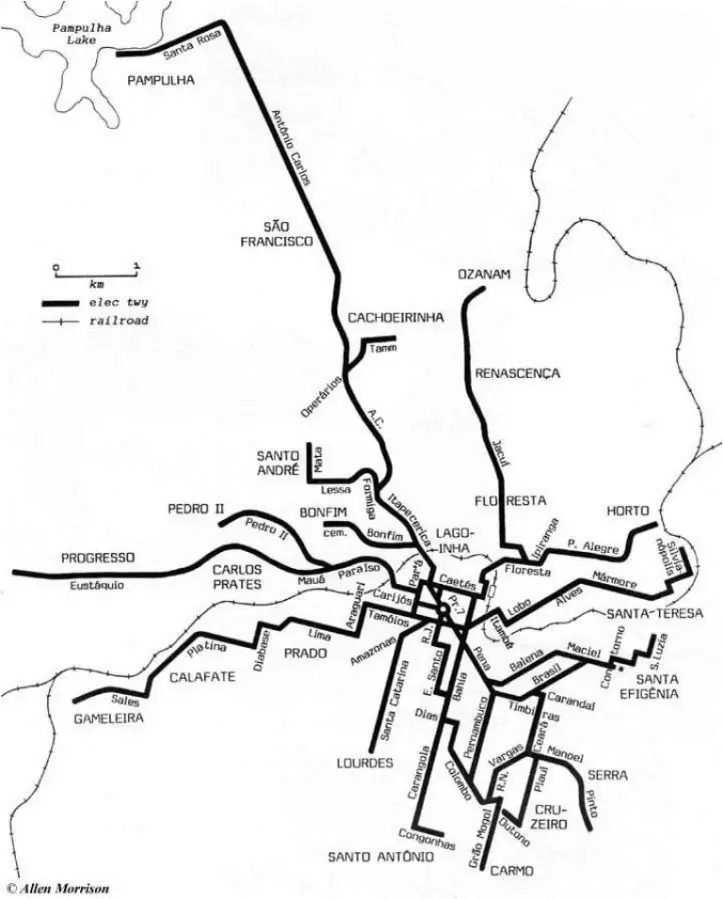
\includegraphics[width=10.04in,height=0.4\textheight]{src/images/bonde_bh} 

}

\caption{\label{fig:bonde} Rede de bondes em Belo Horizonte, ca. 1950}\label{fig:bonde}
\end{figure}

\begin{quote}
Curiosidade: Diversas manifestações culturais imortalizaram os meios de
transporte. Uma delas é o samba ``O Bonde de São Januário'', de 1940,
que retrata o trajeto de operários que trabalhavam no bairro de São
Cristóvão (próximo ao centro do Rio de Janeiro).
\end{quote}

\hypertarget{inovauxe7uxf5es-nas-tuxe9cnicas-de-construuxe7uxe3o}{%
\subsubsection{Inovações nas técnicas de
construção}\label{inovauxe7uxf5es-nas-tuxe9cnicas-de-construuxe7uxe3o}}

Outra restrição importante para a estrutura urbana é a
\textbf{tecnologia construtiva} disponível. Até o início do século XIX,
raras construções passavam do limite de \textbf{três andares}, pois as
estruturas baseadas em madeira e barro não permitiam ir muito além. Com
isso, mesmo que houvesse forças econômicas na direção do adensamento,
este encontrava uma \textbf{barreira técnica}.

Com o barateamento de \textbf{pregos} e o surgimento de estruturas em
\textbf{metal}, foi possível atingir novos patamares. Esse processo foi
impulsionado pela invenção do \textbf{elevador}, em 1853, que tornou os
pisos superiores atrativos ---afinal, quando só haviam escadas, estes
tinham acessibilidade inferior. O elevador chegou a inverter a lógica de
\textbf{valorização fundiária}: se antes o térreo era mais valorizado,
com o elevador, os pisos superiores foram apreciados, pelas suas
amenidades (vista e circulação de ar).

Assim, o desenvolvimento dos métodos construtivos permitiu um
\textbf{maior adensamento} das cidades onde havia vantagens locacionais,
tanto residenciais quanto comerciais. Isso reforça o padrão
\textbf{monocêntrico}; graficamente, torna o gradiente de densidade
\textbf{mais inclinado} (como Paris e Pequim, na Figura 1, em contraste
com Atlanta e Los Angeles).

\hypertarget{o-decluxednio-da-cidade-monocuxeantrica}{%
\section{O declínio da cidade
monocêntrica}\label{o-decluxednio-da-cidade-monocuxeantrica}}

Até aqui, vimos que no princípio as indústrias se localizavam coladas ao
centro e aos portos pela dificuldade de locomoção. Posteriormente, as
ferrovias permitiram novos padrões de organização da indústria no
espaço, mas ainda de forma limitada: afinal, da fábrica para as
estações, ainda era necessário transportar as mercadorias por carroças.
Esse cenário mudou com o surgimento do \textbf{caminhão}, nos anos 1900,
ao facilitar enormemente o deslocamento de mercadorias, por ser mais
rápido e ter maior volume.

Eventualmente, o caminhão se tornou \textbf{competitivo} frente aos
trens e embarcações para o transporte interurbano, com um impacto forte
no tecido urbano por dois motivos. Primeiro, como não estavam mais
restritas à vizinhança do centro, das estações ferroviárias e dos
portos, a localização ótima para várias firmas passou a ser na
\textbf{periferia}, onde a terra era mais barata, mas ainda ao alcance
da oferta de trabalho.

A teoria nos ajuda a entender a decisão locacional da firma. Os painéis
da figura abaixo ilustram um modelo similar ao que vimos na Aula 6, em
que os \textbf{custos de frete} aumentam à medida que a empresa se
distancia do porto (e se aproxima da residência dos trabalhadores) e o
custo com \textbf{mão de obra} cresce na direção \textbf{contrária}.

\begin{figure}

{\centering 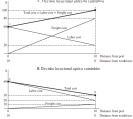
\includegraphics[width=21.88in]{src/images/caminhao_2} 

}

\caption{\label{fig:caminhao} decisão locacional. Fonte: O'Sullivan (2012)}\label{fig:caminhao}
\end{figure}

\textbf{Antes} da popularização do caminhão (painel A), o custo de
\textbf{frete era proibitivo} o bastante que a decisão racional
(minimizadora de custos) fosse instalar a planta junto ao porto.
\textbf{Após o caminhão} (painel B), o custo de frete cai drasticamente.
Note que o custo de trabalho é o mesmo; todavia, como a curva do custo
de frete não cruza com a outra, a decisão racional é instalar a unidade
junto à fonte de mão de obra. Na prática, a decisão ótima varia, mas o
gráfico ilustra bem o processo de \textbf{desconcentração das
indústrias} que se segiu.

\hypertarget{carros-rodovias-e-o-rodoviarismo}{%
\subsubsection{Carros, rodovias e o
rodoviarismo}\label{carros-rodovias-e-o-rodoviarismo}}

Se na indústria o caminhão proporcionou uma revolução na distribuição
espacial, os carros lideraram o mesmo processo no lado das residências.
A popularização do automóvel representou um ganho de acessibilidade para
várias pessoas, na medida em que não se viam mais restritas aos horários
do transporte público e aos corredores por onde eles passavam. Uma
consequência direta no equilíbrio espacial urbano é que regiões com
pouca ou nenhuma oferta de transporte coletivo se tornaram valorizadas.
Locais afastados se transformaram em bairros residenciais com pouca ou
nenhuma verticalização, consequência direta do \textbf{investimento em
rodovias} e na indústria automobilístico, sobretudo após a II Guerra
Mundial.

Esse processo foi mais intenso nos Estados Unidos, mas também ocorreu na
Europa e na América Latina. Tratava-se de uma \textbf{mudança de
paradigma} no pensamento urbanístico: não apenas os carros eram vistos
com o o meio de transporte do futuro, como as políticas de
\textbf{urbanização} refletiam um espaço urbano \textbf{voltado para o
fluxo de automóveis}. Um exemplo claro é Brasília, desenvolvida no auge
do pensamento rodoviarista, cidade até hoje marcada pelas longas
distâncias e baixa atratividade ao pedestre.

\hypertarget{economia-da-informauxe7uxe3o-e-outros-fatores}{%
\subsubsection{Economia da informação e outros
fatores}\label{economia-da-informauxe7uxe3o-e-outros-fatores}}

Até os anos 1970, o contato físico era indispensável para várias
atividades que hoje podem ser feitas de forma remota, automática, ou
sequer existem. Relatórios gerenciais, demonstrativos contábeis,
cálculos de engenharia eram essencialmente manuais, e a informação,
transmitida sobretudo por \textbf{papel}. Dada essa natureza, era
racional que as firmas alocassem essas \textbf{atividades técnicas em
áreas centrais}, para que a \textbf{comunicação e tomada de decisão
fluísse}. No entanto, o fluxo de inovações na informática
---microcomputador, internet, email, planilhas, videoconferência,
smartphone--- tornaram o contato físico cada vez menos importante.
Várias atividades foram deslocadas para regiões menos nobres ou para o
modelo de \emph{home office}; por outro lado, atividades que envolvem
\textbf{liderança} e informações tácitas, como reuniões de negócios,
seguem sendo desempenhadas em \textbf{locais centrais}.

Outros fatores também diminuíram a pressão sobre os centros. Um deles é
o surgimento de processos produtivos, como o fordismo e o toyotismo, que
aumentaram a preferência por indústrias \textbf{horizontais} em vez das
plantas multipavimento: como a terra costuma ser mais barata na
periferia, foi mais um incentivo para que as indústrias saíssem da
região central e se agrupassem em \textbf{novas centralidades}. Outro
fator foi o desenvolvimento da aviação e de produtos de alto valor que
passaram a a ser transportados por via aérea. Assim, nas proximidades
dos aeroportos surgiram novos clusters de indústrias e atividades
econômicas de suporte.

\hypertarget{espraiamento-causas-e-consequuxeancias}{%
\section{Espraiamento: causas e
consequências}\label{espraiamento-causas-e-consequuxeancias}}

Como vimos na seção anterior, o desenvolvimento dos meios de transporte
incentivOU que as cidades crescessem para os lados, por tornar os
deslocamentos mais rápidos. Novas técnicas construtivas resultaram no
adensamento, ao possibilitarem que cada vez mais pessoas ocupassem
espaços valiosos. Essa combinação de forças \textbf{reforçou o caráter
monocêntrico} dos centros urbanos. Por sua vez, a ascenção do automóvel,
a priorização do transporte individual nas políticas urbanas, a
revolução propiciada pela informática e outros fatores diminuíram cada
vez mais a pressão sobre as áreas centrais e levaram à
\textbf{descentralização} do espaço urbano. Ao mesmo tempo, a expansão
dos limites urbanos se intensificou. Nesta seção, examinaremos o
\textbf{espraiamento} ---processo de urbanização de regiões até então
rurais ou desocupadas---, fenômeno bastante relacionado ao processo de
descentralização do tecido urbano.

\begin{quote}
Exemplo de espraiamento: entre os anos 1950 e 1990, os centros urbanos
dos Estados Unidos se expandiram em 245\%, enquanto a população cresceu
em 92\% (O'Sullivan 2012).
\end{quote}

\hypertarget{causas-do-espraiamento}{%
\subsection{Causas do espraiamento}\label{causas-do-espraiamento}}

Em primeiro lugar, analisemos os motores do espraiamento no lado da
demanda. De acordo com os modelos de economia urbana, a \textbf{terra é
um bem normal}; ou seja, sua derivada em relação à renda é maior que
zero. Na maioria dos países que passam pelo processo de espraiamento nos
últimos 60 anos, a \textbf{renda média} familiar se elevou bastante:
assim, tudo o mais constante, a escolha maximizadora de diversos
consumidores foi consumir \textbf{propriedades maiores}. Esse processo
de enriquecimento se deu, em diversos países (inclusive no Brasil), ao
mesmo tempo em que o desenvolvimento dos automóveis e das rodovias
tornaram locais distantes mais atrativos. Pensando nos modelos que

\hypertarget{consequuxeancias-do-espraiamento}{%
\subsection{Consequências do
espraiamento}\label{consequuxeancias-do-espraiamento}}

\hypertarget{referuxeancias}{%
\section*{Referências}\label{referuxeancias}}
\addcontentsline{toc}{section}{Referências}

\hypertarget{refs}{}
\begin{CSLReferences}{1}{0}
\leavevmode\vadjust pre{\hypertarget{ref-bertaud2018}{}}%
Bertaud, Alain. 2018. \emph{Order without design: how markets shape
cities}. Cambridge, Massachusetts: MIT Press.

\leavevmode\vadjust pre{\hypertarget{ref-bertaud2003}{}}%
Bertaud, Alain, e Stephen Malpezzi. 2003. {"The Spatial Distribution of
Population in 48 World Cities: Implications for Economies in
Transition"}, dezembro, 103.

\leavevmode\vadjust pre{\hypertarget{ref-brueckner2011}{}}%
Brueckner, Jan K. 2011. \emph{Lectures on Urban Economics}. Cambridge,
Mass: MIT Press.

\leavevmode\vadjust pre{\hypertarget{ref-osullivan2012}{}}%
O'Sullivan, Arthur. 2012. \emph{Urban Economics}. 8th ed. New York, NY:
McGraw-Hill/Irwin.

\end{CSLReferences}

\end{document}
